\documentclass[tikz]{standalone}
\usepackage{fontspec}
\renewcommand*{\familydefault}{\sfdefault}
\usepackage{standalone}
\usepackage{amssymb}
\usetikzlibrary{decorations}
%\usetikzlibrary{arrows.meta, decorations.pathmorphing, decorations.pathreplacing, shapes.geometric}
\usetikzlibrary{bayesnet}

\begin{document}
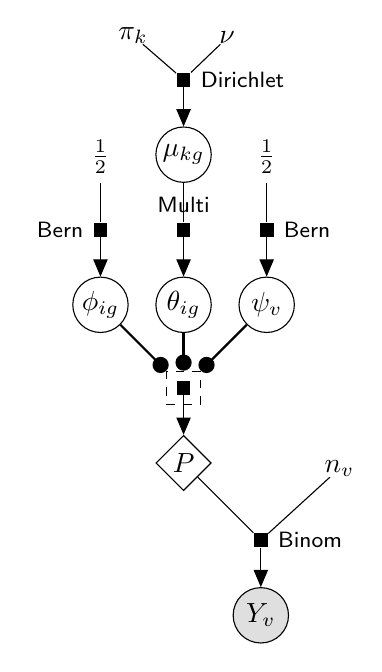
\begin{tikzpicture}%[font=\footnotesize, xscale=1.5]


    % bottom level (closest to observed Y)
    \node[obs] (Y) {\(Y_v\)};
    \factor[above=0.5 of Y, label=right:Binom] {Y-factor} {} {} {};
    \node[det, above left=1.0 of Y-factor] (P) {\(P\)};
    \node[const, above right=1.0 of Y-factor] (n) {\(n_v\)};
    \factoredge {P, n} {Y-factor} {Y};


    % middle level
    % regression coefficients and explanatory variables
    \factor[above=0.5 of P] {P-factor} {} {} {};
    \node[latent, above left=1.0 of P-factor] (phi) {\(\phi_{ig}\)};
    \node[latent] (theta) at (phi -| P) {\(\theta_{ig}\)};
    \node[latent, above right=1.0 of P-factor] (psi) {\(\psi_{v}\)};
    \gate {mygate} {(P-factor)} {phi, theta, psi};
    \factoredge {} {P-factor} {P};


    % higher level
    % phi
    \factor[above=0.5 of phi, label=left:Bern] {phi-factor} {} {} {};
    \node[above=0.5 of phi-factor] (phi-param) {\(\frac{1}{2}\)};
    \factoredge {phi-param} {phi-factor} {phi};
    % theta
    \factor[above=0.5 of theta, label=90:Multi] {theta-factor} {} {} {};
    \node[latent, above=0.5 of theta-factor] (mu) {\(\mu_{kg}\)};
    \factoredge {mu} {theta-factor} {theta};
    % psi
    \factor[above=0.5 of psi, label=right:Bern] {psi-factor} {} {} {};
    \node[above=0.5 of psi-factor] (psi-param) {\(\frac{1}{2}\)};
    \factoredge {psi-param} {psi-factor} {psi};


    % top level
    \factor[above=0.5 of mu, label=right:Dirichlet] {mu-factor} {} {} {};
    \node[const, above left=0.5 of mu-factor] (pi) {\(\pi_{k}\)};
    \node[const, above right=0.5 of mu-factor] (nu) {\(\nu\)};
    \factoredge {pi, nu} {mu-factor} {mu};

    % plate
    %\plate {v-plate} {(Y) (n) (psi)} {\(v\in(i,g)\)};

\end{tikzpicture}
\end{document}
